\documentclass[a4paper,twoside]{article}

\usepackage{epsfig}
\usepackage{subfigure}
\usepackage{calc}
\usepackage{amssymb}
\usepackage{amstext}
\usepackage{amsmath}
\usepackage{amsthm}
\usepackage{multicol}
\usepackage{pslatex}
\usepackage{apalike}
\usepackage{SCITEPRESS}     % Please add other packages that you may need BEFORE the SCITEPRESS.sty package.

\subfigtopskip=0pt
\subfigcapskip=0pt
\subfigbottomskip=0pt

\begin{document}

\title{Ontology Based Description of Analytic Methods for Electrophysiology}

\author{\authorname{Jan Stebetak, Roman Moucek}
\affiliation{Department of Computer Science and Engineering, University of West Bohemia, Univerzitni 8, Pilsen, Czech Republic}
\email{\{stebjan, moucek\}@kiv.zcu.cz}
}

\keywords{neuroinformatics, electroencephalography, event-related potentials, analytic methods, metadata, semantic web, ontology}

\abstract{The growing electrophysiology research leads to the collection of large amounts of experimental data and consequently to the broader application, eventually development of analytic methods, algorithms, and workflows. Then appropriate metadata definition and related data description is critical for long term storage and later identification of experimental data. Although a detailed description of electrophysiology data has not become a commonly used procedure so far, publicly available and well described data have started to appear in professional journals. The next reasonable step is to shift attention to the analysis of electrophysiology data. Since the analysis of this kind of data is rather complex, identification and appropriate description of used methods, algorithms and workflows would help reproducibility of the research in the field. This description would also allow developing automatic or semi-automatic systems for data analysis or constructing complex workflows in a more user friendly way. Based on these assumptions authors present a custom ontology for description of analytic methods and workflows in electrophysiology that is proposed to be discussed within the scientific community.}

\onecolumn \maketitle \normalsize \vfill

\section{\uppercase{Introduction}}
\label{sec:introduction}

\noindent Our research group at [anonymous%University of West Bohemia in Pilsen]
specializes in the research of human brain activity. We use the methods and techniques of electroencephalography (EEG) and event-related potentials (ERP). As the electrophysiology research grows, larger amounts of data are collected and more complex methods and workflows are used for data analysis. Typically, electrophysiology workflows used in our laboratory include preprocessing methods (e.g. filtering, baseline correction), signal processing methods (for example feature extraction methods, clustering and classification methods), and postprocessing (usually statistical) methods. To make the application of complex analytic methods and workflows reproducible, a need for identification and sharing of their appropriate descriptions arises. These descriptions would also allow developing automatic or semi-automatic systems for data analysis or constructing complex workflows in a more user friendly way. Then by defining proper metadata structures for analytic methods and workflows and by using suitable technologies for machine-processing the workflow systems can ensure the following procedures:

\begin{itemize}
	\item Checking the syntactic compatibility of methods (the output of the previous method is supplied as an input to the following method)
	
	\item Checking the semantic compatibility of methods (connection of methods makes sense in terms of their semantic and also semantic of their output and input)
	
	\item Suggesting, which method is suitable to put next into workflow
	
\end{itemize}

\item to check the syntactic compatibility of the used methods (the output of the previous method is used as an input to the following method
\item to check the semantic compatibility of the used methods (connection of methods has sense in terms of their semantic usage within the processing chain and also semantic compatibility of transferred parameters)
\item to suggest, which method is suitable to be put next into the workflow

In this paper, we present a definition of the metadata structure that describes the methods used in analytic processing of electrophysiology data in our laboratory. This structure thus helps to identify the semantic compatibility of the methods while constructing workflows. The rest of this paper is organized as follows: Section II describes the analytic methods that we use for processing of electrophysiology data. It also briefly presents the Semantic web technologies and existing ontologies. Section III deals with the metadata definition. The selection of a suitable technology is provided in Section IV and the proposed ontology is presented in Section V. This section is followed by conclusions and future work description.

\section{\uppercase{State of the Art}}

\noindent This section brings an overview of existing approaches to description of analytic methods and workflows. Then it introduces the analytic methods suitable for electrophysiology research that we use for data analysis in our laboratory. Then the Semantic web technologies are briefly described.

\subsection{Existing Approaches}

The CARMEN Portal \cite{Watson07} (Code Analysis, Repository \& Modelling for e-Neuroscience) developed by the British National Node allows neuroscientists to save and share experimental data and services. CARMEN provides storage of services. There is a number of public services available such as data filters, neural spike detection and spike sorting methods. No formal semantics or metadata structures are used for description of these methods, they are described in a natural language.

The Galaxy project \cite{goecks2010galaxy, blankenberg2010galaxy, giardine2005galaxy} is an open source workflows engine. A registered user is able to use methods and workflow tools provided by this system. Galaxy is focused on genome analysis; therefore, this system contains methods suitable for genome analysis. The methods are well described for the users with description of parameters and examples. It also includes OBI ontology (ontology for biomedical investigation) for formal description of semantic restrictions.

The Wings is an open source workflows engine (its source code is available at GitHub) and portal based system downloadable and runnable on local servers. The methods the engine works with are described by ontologies (in the Resource Description Framework). This description includes definition of semantic constraints such as allowed values, input/output cardinality, range, etc. The main disadvantage is a~small community of developers and annoying bugs (e.g. difficulty with adding a new method into the Wings system) that we found while trying to deploy the system on a server.

This overview shows that the formal description of methods in terms of semantic constraints (e.g. allowed values) exists. However, the proper description of input/output parameters allowing semantic comparison of methods is still not satisfactorily solved. Therefore, we propose description of methods that allows such comparison in this paper.

\subsection{Analytic Methods}

\noindent In our laboratory we widely use the following signal preprocessing and processing methods: averaging, FIR filters, Matching Pursuit, Discrete and Continuous Wavelet transform, Fast Fourier transform, Hilbert-Huang transform, and various neural networks. This section briefly describes the basic principles of these algorithms since metadata definitions that follow will be proposed just for these methods. We admit that the methods described in this paper are only a subset of a larger set of methods that can be used in signal preprocessing and processing. This is taken into account and the proposed design will allow straightforward extension of metadata definitions.

Averaging \cite{Sanei07} is a common method for highlighting ERP waveforms. During the averaging of  the  same  kind  of  ERP  waveforms,  the  noise  is  reduced  and  the  waveform  is  highlighted. Since the background  EEG  has a higher  amplitude  then  ERP  waveforms, the averaging technique highlights the waveforms and suppress the background EEG \cite{Vidal77}.

The Matching Pursuit method has been frequently used for continuous EEG processing. It decomposes any signal into a linear expansion of functions. At each iteration, a waveform is chosen in order to best match the
significant structures of the signal. Typically, this part is approximated by a Gabor atom, which has the highest scalar product with the original signal, and then it is subtracted from the signal. This process is repeated until the whole signal is approximated by Gabor atoms with an acceptable error \cite{Vareka12}. For displaying results we implemented the time-frequency transformation known as Wigner-Ville transformation \cite{Quian02}. The input of this transformation is the set of chosen atoms.

Wavelet Transformation (WT) \cite{Ciniburk10} is a suitable method for analyzing and processing non-stationary signals such as EEG. WT has a good time and frequency localization, which is necessary for ERP detection. For EEG signal processing it is possible to use Continuous Wavelet Transformation or Discrete Wavelet Transformation. For visualization of wavelet results, the scalogram (Figure 1) is used.

\begin{figure}[!h]

  \centering
   {
\epsfig{file = scalogram.eps, width = 7.3cm}}
  \caption{Input signal and its scalogram. \cite{Rondik12} }
  \label{fig:scalogram}
 \end{figure}

The Fourier transform converts waveform data in the time domain into the frequency domain. Since artifacts usually have higher amplitude and basic frequency than a normal ERP component, this technique is useful for detecting artifacts within the EEG or ERP signal.

Independent Component Analysis (ICA) \cite{Hyv01} is a method for blind signal separation and signal deconvolution. In the EEG/ERP domain, ICA can be used for artifact removal, ERPs detection, and, generally speaking, for detection and separation of every signal which is independent on EEG activity.

The  Hilbert-Huang  transform  (HHT)  was  designed  to  analyze  nonlinear  and  non-stationary signal. This also includes detection of ERP waveforms that is described in \cite{Ciniburk11}.

\subsection{Semantic Web Technologies}

\noindent The Semantic Web is a layered architecture. The first layer is called Resource Description Framework (RDF). RDF is a simple metadata representation framework using URIs to identify web-based resources and a graph model for describing relationships between resources. Web ontology language (OWL) is a semantically richer language and provides more complex constraints on the types of resource and their properties. OWL comes with a larger vocabulary, greater machine interpretability and stronger syntax than RDF.

There are substantial differences between classic object-oriented languages such as Java or C\# and Semantic Web technologies. The semantics of classes and instances in RDF Schema is open-world and description logics-based while object-oriented type systems are closed-world and constraint-based \cite{Kalyanpur02}. The following list brings main differences between OOP and Semantic web \cite{Oren07}

\begin{itemize}

\item class membership: in object-oriented languages, an object is a member of exactly one class: its membershi is fixed and is defined during the object instantiation. In RDF Schema, a resource can belong to multiple classes: its membership is not fixed but defined by its rdf:type and the properties that belong to the resource.

\item class hierarchy: in object-oriented type systems, classes can usually inherit from one superclass, while in RDF Schema classes can inherit from multiple superclasses.

\item attribute vs. property: in the object-oriented model, attributes are defined locally inside their class, can be used only by instances of that class, and generally have single-typed values. In contrast, RDF properties are stand-alone entities that can be used by any resource of any class and that can have values of different types.

\item structural inheritance: in object-oriented programming, objects inherit their attributes from their parent classes. In RDF Schema, since properties do not belong to a class, they are not inherited.  Instead, property domains are propagated, but given their specific meaning indicating the class membership of resources using that property, domains propagate into the upwards direction of the class hierarchy.

\item object conformance: in most object-oriented languages, the structure of instances must exactly follow the definition of their classes, whereas in RDF Schema, a class definition is not exhaustive and does not constrain the structure of its instances: any RDF resource can use any property.

\item flexibility: object-oriented systems usually do not allow class definitions to evolve during runtime. In contrast, RDF is designed for integration of heterogeneous data with varying structure from varying sources, where both schema and data evolve during runtime.

\end{itemize}

The main advantage of Semantic Web technologies (e.g. RDF or OWL language) is the ability to evolve during runtime. Since newly created or added methods have to be well described, an extendable metadata definition is necessary. Easy reusability of classes and properties is also crucial, therefore the Semantic Web concept and technologies were chosen for description of the analytic methods described above.

\section{\uppercase{Metadata Definition and Ontology Development}}

\noindent Because there is no suitable description of the methods used in electrophysiology, we proposed their semantic description by using a set of metadata. Describing analytic methods at a more specific level for workflow construction requires a detailed analysis of the methods' operations in terms of semantics of their and inputs and outputs.

The metadata identification originated from our experience with data analysis, expertise of co-workers from cooperating institutions, books describing principles of EEG/ERP design and data recording (e.g. \cite{Luck05}), and numerous scientific papers describing processing of EEG/ERP data. We defined the following metadata and their structure:
\begin{itemize}
	\item Method - It describes a method including its name and input/output types. It also includes definitions of restrictions (e.g. name is a string).
	
	\item Input/Output - It describes input/output types used by analytic methods. It includes signal such as EEG or ECG, and its restrictions (e.g. signal has values of double), coefficients from the Wavelet transform, or atom provided by the Matching Pursuit method (the atom is composed of scale, frequency, modulus, phase, and position represented as double values).
	
\end{itemize}

Figure 2 shows the structure of Signal and Atom input/output types.

\begin{figure}[!h]

  \centering
   {\epsfig{file = SignalAndAtom.eps, width = 7.5cm}}
  \caption{a) Structure of Signal as an I/O type, b) Structure of Atom }
  \label{fig:SignalAndAtom}
 \end{figure}

Defining metadata we continued with the development of the ontology for analytic methods introduced in Section 2.2. Table 1 brings an overview of these methods enriched with input/output parameter(s) types.


\begin{table}[h]
\caption{Overview of methods and parameters}\label{tab:example1} \centering
\begin{tabular}{|p{2cm}|p{2cm}|p{2cm}|}
  \hline
  Method name & Input parameter(s) & Output parameter(s) \\
  \hline
  Detection of epochs & EEG signal &  Set of detected epochs \\
  \hline
  Fourier Transform & EEG/ERP signal &  Detected frequencies \\
  \hline
  Wavelet Transform & EEG/ERP signal &  Computed coefficients \\
  \hline
  Matching Pursuit & EEG/ERP signal &  List of selected atoms \\
  \hline
  ICA & EEG/ERP signal &  ICA components \\
  \hline
  Hilbert-Huang Transform & EEG/ERP signal & Set of Intrinsic Mode Functions \\
  \hline
  Neural network & Featured vector & Vector of weights \\
  \hline
\end{tabular}
\end{table}


For the ontology development we used Protege, which is a free, open-source ontology editor and framework for building intelligent systems. The following terms were defined for the semantic group method:
\begin{itemize}
\item Class Method and its named individuals (DetectionOfEpochs, Averaging, CWT, DWT, FFT, FastICA, FIR, and MatchingPursuit)
\item Class IOType representing general input/output type (any class or individual)
\end{itemize}

We also defined properties hasInput and hasOutput. The class Method is a domain class for these properties and the class IOType defines their range. The class IOType has the following subclasses:

\begin{itemize}
\item Class Signal (an example of this class is given below) represents a set of values (signal amplitudes) and individuals such as eegSignal, ecgSignal, ...). Epoch, FilteredSignal, and ReconstructedSignal are subclasses of this class. For these classes we defined an object property hasSignalValue, which range is the class SignalValue leading to a data property named Value with the defined type xsd:double.

\item Class Coefficient represents a generic type for a coefficient (for classes in this list that include coefficients as their object properties). The coefficient value defined as object property is of the double value.

\item Classes CWTCoefficients and DWTCoefficients are computed coefficients that represent the return type of the methods Continuous Wavelet Transform resp. Discrete Wavelet Transform.

\item Class ComplexFrequency represents composition of RealFrequency and ImaginaryFrequency classes. This type is typically used as an output of time-frequency analytic methods such as Fast Fourier Transform. It has two object properties: hasRealValue and hasImaginaryValue. The properties range are RealValue class resp. ImaginaryValue class.

\item Class Atom represents the output type of the Matching Pursuit method. It includes five coefficient types (classes Frequency, Scale, Modulus, Position, and Phase) and five corresponding object properties (hasFrequency,...).
\end{itemize}

Below an RDF example containing the class Signal, the object property hasSignalValue, and the data property Value is shown.

\begin{small}
\begin{verbatim}
<owl:Class rdf:about=
"http://www.semanticweb.org/eegMethods#Signal">
  <rdfs:subClassOf>
    <owl:Restriction>
      <owl:onProperty rdf:resource=
        "http://www.semanticweb.org/
        eegMethods#hasSignalValue"/>
      <owl:onClass rdf:resource=
        "http://www.semanticweb.org/
        eegMethods#SignalValue"/>
      <owl:minQualifiedCardinality
        rdf:datatype="&xsd;
        nonNegativeInteger">1
      </owl:minQualifiedCardinality>
    </owl:Restriction>
  </rdfs:subClassOf>
</owl:Class>
\end{verbatim}
\end{small}

\begin{small}
\begin{verbatim}
<owl:ObjectProperty rdf:about=
"http://www.semanticweb.org/
eegMethods#hasSignalValue">
  <rdfs:domain rdf:resource=
    "http://www.semanticweb.org/
    eegMethods#ICAComponent"/>
  <rdfs:domain rdf:resource=
    "http://www.semanticweb.org/
    eegMethods#Signal"/>
  <rdfs:range rdf:resource=
    "http://www.semanticweb.org/
    eegMethods#SignalValue"/>
</owl:ObjectProperty>
\end{verbatim}
\end{small}

\begin{small}
\begin{verbatim}
<owl:DatatypeProperty rdf:about=
"http://www.semanticweb.org/eegMethods#Value">
  <rdfs:domain rdf:resource=
    "http://www.semanticweb.org/
    eegMethods#CoefficientValue"/>
  <rdfs:domain rdf:resource=
    "http://www.semanticweb.org/ontologies/
    eegMethods#SignalValue"/>
  <rdfs:range rdf:resource="&xsd;double"/>
</owl:DatatypeProperty>
\end{verbatim}
\end{small}

\noindent Figure 3 shows a tree of defined classes provided by the Protege.

\begin{figure}[!h]

  \centering
   {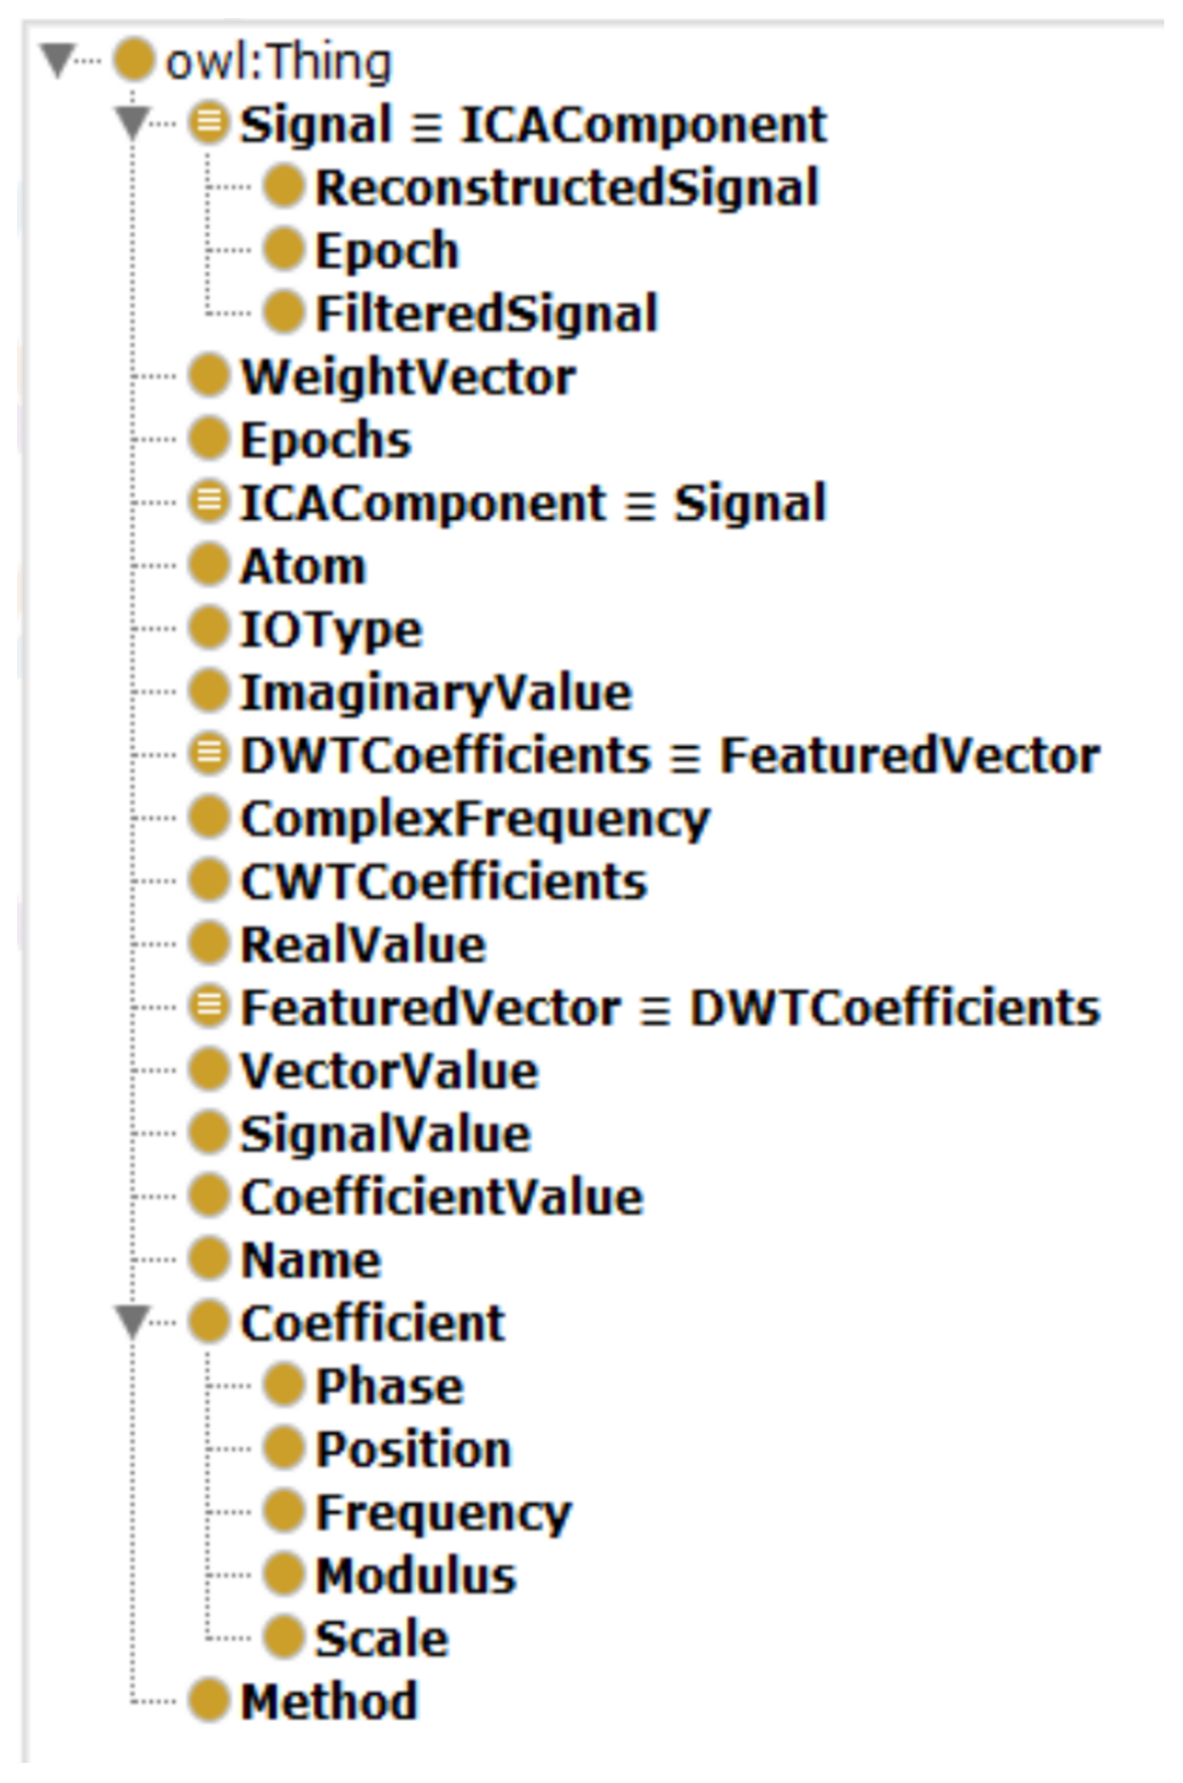
\epsfig{file = classTree.eps, width = 6 cm}}
  \caption{Tree of classes in Protege}
  \label{fig:classTree}
 \end{figure}

\section{\uppercase{Conclusions}}
\label{sec:conclusion}

\noindent This paper summarizes methods suitable for EEG/ERP signal
preprocessing and processing. It brings an introduction
to principles of these methods as well as their using
for ERP waveforms detection or artifacts removal.

Since complex data analyses often require using multiple methods sequentially, it is crucial to find suitable methods to achieve a goal. Therefore, we defined the set of metadata describing methods suitable for electrophysiology research.

Adding semantics to the methods in form of metadata allows checking both syntactic and semantic compatibility. Using the Semantic web technologies also enables processing metadata by machines. Therefore, we develop the ontology includes defined metadata. This brings an ability to develop automatic or semi-automatic workflow systems.

The presented ontology is also easily extendable. It allows reusing existing classes and properties, it also enables defining new classes and/or properties when necessary.

\subsection{Future Work}
\noindent We will annotate the input/output parameters of our methods with the terms defined in the ontology. It allows us to ensure the compatibility of methods while constructing workflows.

We also plan to develop a workflow suggestion system based on the presented ontology that will help users to find suitable methods while constructing workflows.


\section*{\uppercase{Acknowledgements}}

\noindent The work was supported by the UWB grant SGS-
2013-039 Methods and Applications of Bio- and
Medical Informatics.


\vfill
\bibliographystyle{apalike}
{\small
\bibliography{HEALTHINF2016}}



\vfill
\end{document}

